\section{Comment représenter les données spatiales
?}\label{comment-repruxe9senter-les-donnuxe9es-spatiales}

Pour rappel, le TD d'introduction sur la collecte de données est en
ligne à cette adresse :
\url{https://github.com/nkarasiak/1A_DATA-COLLECT}

\subsection{Objectif du TD}\label{objectif-du-td}

L'objectif de ce TD est de vous faire produire des cartes selon la
sémiologie graphique en vigueur c'est-à-dire, les règles graphiques à
respecter pour bien représenter vos données.

\subsection{Télécharger les
données}\label{tuxe9luxe9charger-les-donnuxe9es}

Les données utilisées pour ce TD sont disponibles à cette adresse :
\url{https://github.com/nkarasiak/1A_DATA-VISU/archive/data.zip}.

\subsection{Les principaux types de données à
représenter}\label{les-principaux-types-de-donnuxe9es-uxe0-repruxe9senter}

\begin{itemize}
\tightlist
\item
  Une \textbf{variable quantitative absolue} dont la valeur dépend de la
  surface de l'objet spatial à laquelle elle est associée (ex : nombre
  d'habitants par ville). Dans ce cas, les règles de sémiologie
  graphique préconisent d'utiliser la \textbf{taille} comme
  \emph{variable visuelle} et de passer en mode d'implantation
  ponctuelle à l'aide de
  \href{https://www.geoclip.fr/portfolio-item/carte-a-symboles-proportionnels/}{cercles
  proportionnels}. La taille permet d'exprimer graphiquement des
  variations de quantités (relation de proportionnalité), en plus des
  relations de hiérarchie et de différence (i.e.~les 3 messages
  cartographiques pour ce type de variable).
\end{itemize}

\begin{figure}[htbp]
\centering
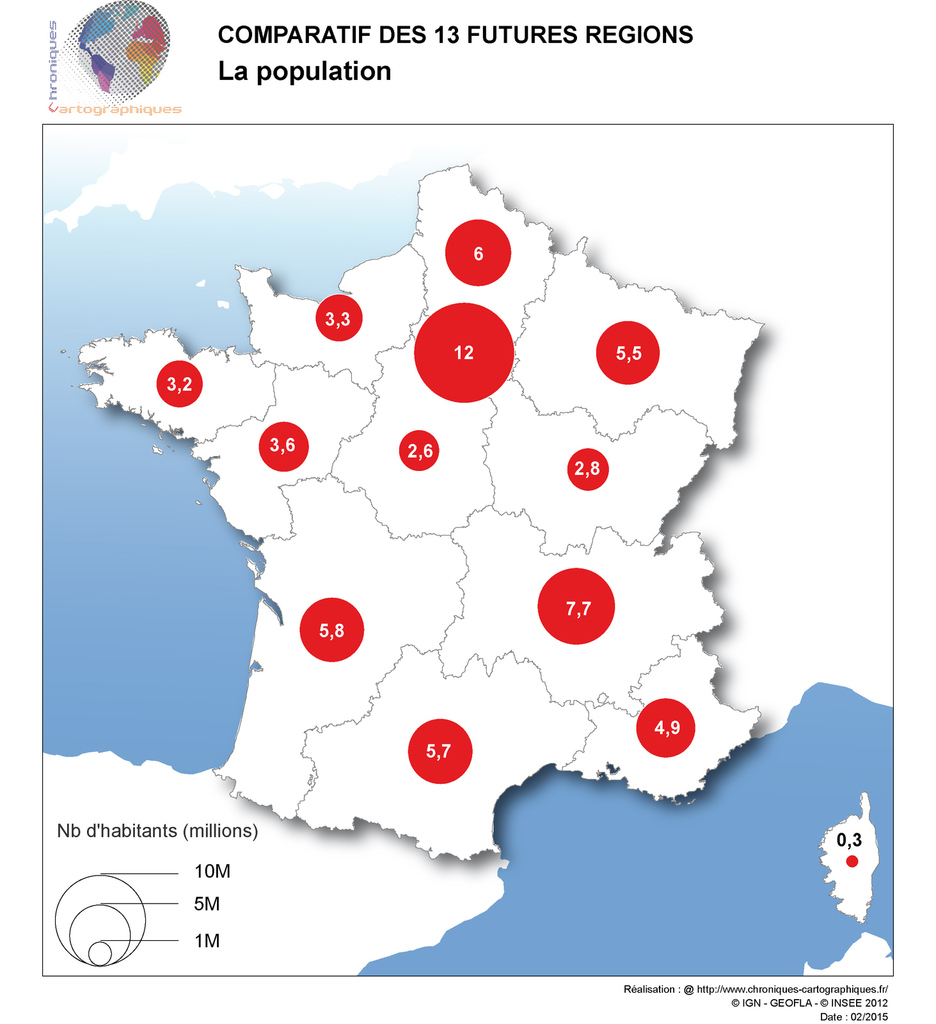
\includegraphics{figures/example_proportion.jpg}
\caption{Représenter une information quantitative de surface variable}
\end{figure}

\begin{itemize}
\tightlist
\item
  Une \textbf{variable quantitative relative} dont la valeur est ramenée
  par unité de surface (ex : une densité - nombre d'habitants par km/2).
  Dans ce cas, les règles de sémiologie graphique préconisent d'utiliser
  notamment la \textbf{valeur} (rapport noir/blanc) comme \emph{variable
  visuelle} sans nécessairement changer de mode d'implantation. La
  valeur permet d'exprimer graphiquement des relations de hiérarchie et
  de différence mais pas de proportionnalité. On construit ainsi des
  \href{https://fr.wikipedia.org/wiki/Carte_choropl\%C3\%A8the}{cartes
  choroplèthes} à l'aide d'un aplat de couleur dont l'intensité varie ou
  à l'aide d'une trame particulière dont la densité de motifs évolue :
\end{itemize}

\begin{figure}[htbp]
\centering
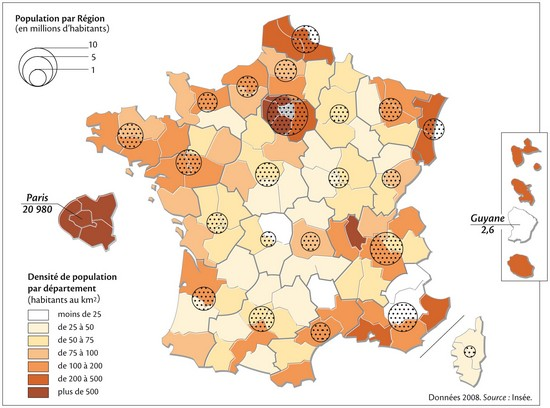
\includegraphics{figures/example_proportion_and_cho.jpg}
\caption{Combinaison de symboles proportionnels avec un dégradé de
couleurs (variation de valeur) pour les informations quantitatives
relatives à la surface}
\end{figure}

\begin{itemize}
\tightlist
\item
  Une \textbf{variable qualitative nominale} en mode d'implantation
  surfacique. Le message cartographique consiste alors à exprimer des
  équivalences ou des différences. Pour cela, on utilise généralement la
  \textbf{couleur} comme \emph{variable visuelle} pour ses propriétés
  d'associativité et de sélectivité.
\end{itemize}

\begin{figure}[htbp]
\centering
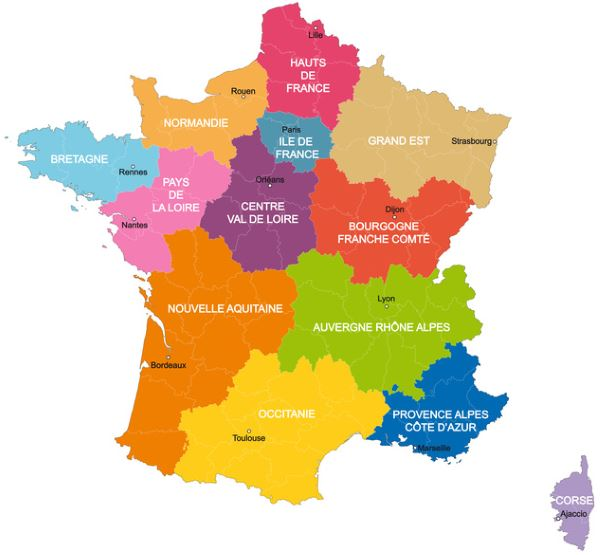
\includegraphics{figures/examples_regions.jpg}
\caption{Différentes régions de la France}
\end{figure}

En mode d'implantation ponctuelle, on aura plutôt recours à la
\emph{variable visuelle} de \textbf{forme} pour exprimer les différences
à l'aide de symboles variés.

\begin{figure}[htbp]
\centering
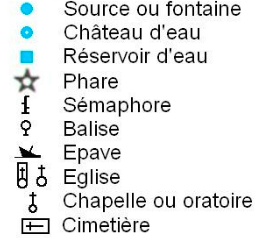
\includegraphics[height=1.04167in]{figures/examples_ponctuel_ign.png}
\caption{Aperçu de la sémiologie ponctuelle de la carte de l'IGN}
\end{figure}

\section{Créer un nouveau projet
QGIS}\label{cruxe9er-un-nouveau-projet-qgis}

Quand vous lancez QGIS, commencez par créer un nouveau projet :
\texttt{Projet\ \textgreater{}\ Nouveau}.

\subsection{Choisir une projection
adaptée}\label{choisir-une-projection-adaptuxe9e}

Par défaut, votre projet utilise le système de référence mondial WGS-84
(celui du GPS), nom de code EPSG:4326. Dans QGIS, le système de
référence du projet est toujours affiché en bas à droite de la fenêtre
de QGIS. Vous pouvez donc vérifier votre projection :

\begin{figure}[htbp]
\centering
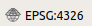
\includegraphics{figures/EPSG4326.png}
\caption{SCR actuel dans QGIS : EPSG:4326}
\end{figure}

Pour regarder les propriétés de votre projet :
\texttt{Projet\ \textgreater{}\ Propriétés}.

Dans l'onglet \texttt{SCR} (Système de Coordonnées de Référence),
recherchez \texttt{2154}, soit le code EPSG de la projection Lambert-93
qui est la projection officielle en France depuis 2000 et obligatoire
pour les données publiques.

Si vous voulez en savoir plus sur cette projection, reportez-vous à la
\href{https://fr.wikipedia.org/wiki/Projection_conique_conforme_de_Lambert}{page
Wikipedia} dédiée.

Une fois la projection Lambert-93 (EPSG:2154) validée, vous pouvez à
nouveau vérifier en bas à droite de la fenêtre de QGIS :

\begin{figure}[htbp]
\centering
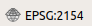
\includegraphics{figures/EPSG2154.png}
\caption{SCR actuel dans QGIS : EPSG:2154}
\end{figure}

Dans l'onglet \texttt{Général}, pensez à donner un nom à votre projet,
il apparaîtra à côté du nom de la fenêtre QGIS.

Une fois ces manipulations effectuées, vous pouvez sauvegarder votre
projet dans votre dossier de travail (ce dossier contiendra également
par la suite vos données vecteur/raster).
\texttt{Projet\ \textgreater{}\ Enregistrer\ sous...}

\subsection{Charger les données}\label{charger-les-donnuxe9es}

Pour ce TD, il est fourni un fichier vectoriel de type polygone où sont
numérisées 10 parcelles de l'exploitation de Borret :
\texttt{parcelles\_borret.gpkg}.

En plus des parcelles, 2 fichiers de type \texttt{csv} sont fournis. Ils
contiennent des données à intégrer aux parcelles :

\begin{itemize}
\tightlist
\item
  \texttt{assolement\_2018.csv}, la liste par parcelle de ce qui a été
  récolté en 2018
\item
  \texttt{rendement.csv}, le rendement (qt/ha) par type de culture
\end{itemize}

\section{Représenter les parcelles}\label{repruxe9senter-les-parcelles}

Dans QGIS 3, il n'y a plus qu'un bouton unique pour ouvrir n'importe
quel type de couche.

\begin{figure}[htbp]
\centering
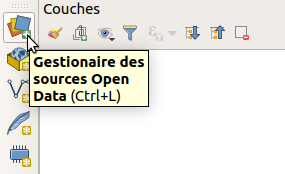
\includegraphics[height=1.56250in]{figures/QGIS_charger.png}
\caption{Charger une couche dans QGIS}
\end{figure}

Une fois le fichier \texttt{parcelles\_borret.gpkg} ouvert, vous pouvez
regarder ce qu'il contient en ouvrant sa table d'attributs
(\texttt{clic\ droit\ sur\ la\ couche\ \textgreater{}\ ouvrir\ la\ table\ d\textquotesingle{}attributs}).

A ce stade, nous pouvons uniquement représenter les informations
contenues dans la table soit les champs \texttt{fid} ou
\texttt{id\_parcelle}.

\subsection{Couleur et étiquette unique par
parcelle}\label{couleur-et-uxe9tiquette-unique-par-parcelle}

Il s'agit de représenter une information qualitative nominale basée sur
la valeur de l'identifiant des parcelles. Chaque parcelle aura ainsi sa
propre couleur.

\subsubsection{Étiquette}\label{uxe9tiquette}

Clic droit \textgreater{} Propriété de la couche \textgreater{}
Étiquettes

\begin{figure}[htbp]
\centering
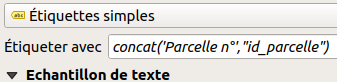
\includegraphics{figures/etiquette_parcelle.png}
\caption{Étiquetter les parcelles}
\end{figure}

Dans étiquettes simples, choisissez le champs content l'identifiant de
la parcelle. N'hésitez pas à changer la police ou à ajouter une ombre
pour mieux voir la police par exemple.

Si vous voulez un texte qui indique `Parcelle n' en plus de la valeur de
son identifiant, il faut \textbf{concatener} deux textes comme suit :

\begin{verbatim}
concat('Parcelle n',"id_parcelle")
\end{verbatim}

Attention à bien mettre des guillemets simples pour ajouter du texte
(sans faire appel à des valeurs d'un champ existant dans la table) et
les double guillemets (``) pour utiliser les champs (comme ici le champs
\texttt{id\_parcelle}).

\begin{figure}[htbp]
\centering
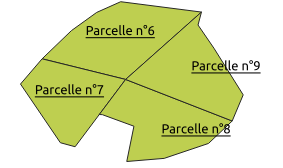
\includegraphics[height=1.56250in]{figures/parcelle_num.png}
\caption{Résultat de l'étiquettage}
\end{figure}

\subsubsection{Couleur (symbologie)}\label{couleur-symbologie}

\begin{figure}[htbp]
\centering
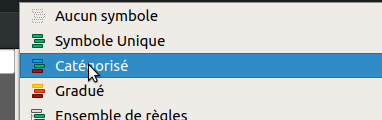
\includegraphics[height=1.04167in]{figures/symbologie.png}
\caption{Liste des symbologies}
\end{figure}

Dans l'onglet symbologie, sélectionnez dans la liste
\texttt{Catégorisé}.

La colonne servant à colorier les parcelles est la même que celle pour
nommer les étiquettes.

Ensuite la ligne \texttt{symbole} vous permet de modifier la façon dont
votre polygone est représenté (style et largeur du contour de votre
polygone par exemple).

Puis, vous pouvez choisir une palette de couleurs. Comme nous sommes sur
une information qualitative nominale et que le message cartographique à
faire passer est une différence, nous choisirons des couleurs
sélectionnées aléatoirement. Vous pouvez désormais cliquer sur le bouton
\texttt{classer} en bas de la fenêtre.

Le rendu est le suivant :

\begin{figure}[htbp]
\centering
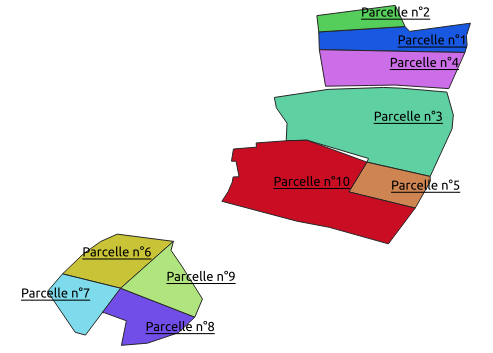
\includegraphics{figures/parcelles_categorise.png}
\caption{Liste des symbologies}
\end{figure}

\subsubsection{Amélioration de la
carte}\label{amuxe9lioration-de-la-carte}

Pour améliorer la beauté de votre carte ;-), vous pouvez par exemple :

\begin{itemize}
\tightlist
\item
  ajouter de la transparence à la couleur de chaque parcelle,
\item
  changer le ligne de contour du polygone,
\item
  changer de police.
\item
  choisir l'endroit où sera placé votre texte
  (\texttt{étiquette\ \textgreater{}\ position\ \textgreater{}\ décalé\ du\ centroïd}
  par exemple)
\end{itemize}

\begin{figure}[htbp]
\centering
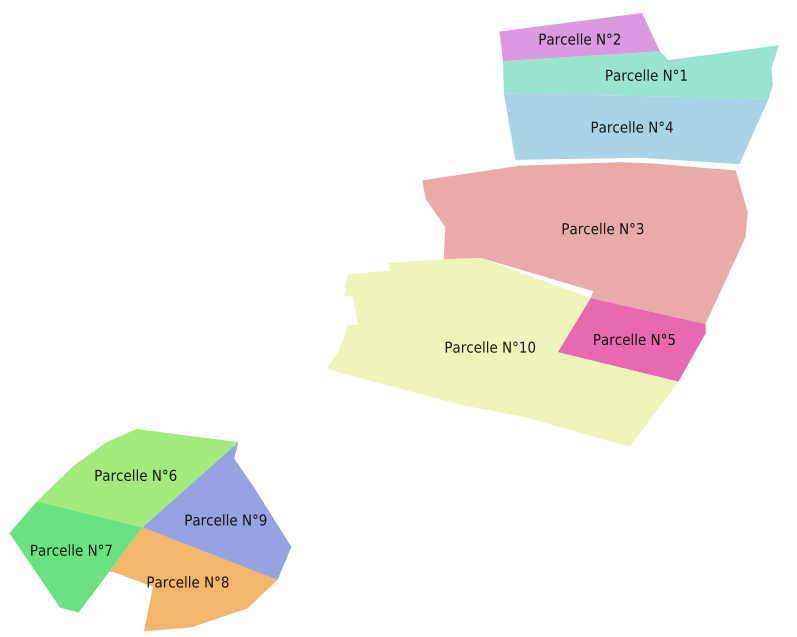
\includegraphics{figures/parcelle_style.png}
\caption{Affichage des parcelles amélioré}
\end{figure}

\section{Créer une carte exportable
(jpg/pdf)}\label{cruxe9er-une-carte-exportable-jpgpdf}

Une fois votre symbologie choisie, vous pouvez créer une mise en page
afin d'y ajouter des éléments essentiels de compréhension comme :

\begin{itemize}
\tightlist
\item
  un titre
\item
  une légende
\item
  le nord
\item
  la localisation sur un planisphère
\end{itemize}

Pour ce faire, aller dans le menu
\texttt{Projet\ \textgreater{}\ Nouvelle\ mise\ en\ page}. Pour ajouter
la carte que vous venez de réaliser dans QGIS, cliquez sur l'icône
\texttt{Ajouter\ une\ carte} dans le menu à gauche.

\begin{figure}[htbp]
\centering
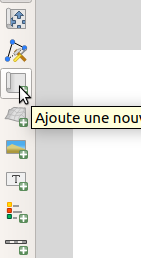
\includegraphics{figures/composer_addMap.png}
\caption{Ajouter une carte}
\end{figure}

Vous pouvez déplacer le contenu de la carte en utilisant l'icône avec
les flêches qui vont dans les 4 sens.

Enfin, si l'emprise de votre carte ne vous satisfait pas, le plus simple
est de retourner dans la fenêtre principale de QGIS puis : clic droit
sur les parcelles, et choisissez ``Zoomer sur la couche'' (autre
solution : modifier l'échelle dans les propriétés de l'objet).

À partir QGIS 3.8, sélectionner votre carte puis cliquer sur l'icône
\texttt{Set\ Map\ Extent\ to\ Match\ Main\ Canvas\ Extent} pour que
votre carte utilise la même emprise que l'emprise de la fenêtre
principale de QGIS. Dans les versions antérieures de QGIS, dans
\texttt{Propriétés\ de\ l\textquotesingle{}objet}, déployez la partie
\texttt{Emprise} puis, cliquez sur
\texttt{Fixer\ sur\ l\textquotesingle{}emprise\ courante\ du\ canevas\ de\ carte}.

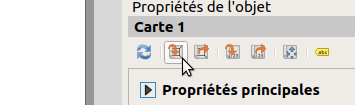
\includegraphics{figures/composer_mapExtent.png}.

Vous pouvez ajouter plusieurs textes : - un titre - les crédits (qui a
fait la carte et avec des données de quelles sources ?).

Et n'oubliez pas d'ajouter une légende (icône légende) et une flèche
nord (icône fléche nord). Si vous n'avez pas d'icône flèche du nord (cet
icône est présent à partir de la version de QGIS 3.8), il vous faut
ajouter une image, puis déployer la partie
\texttt{Recherche\ dans\ les\ repertoires} et enfin sélectionner votre
flèche nord préférée.

Quand la carte vous convient, faites
\texttt{Mise\ en\ page\ \textgreater{}\ Exporter\ au\ format\ PDF},
\texttt{image} ou \texttt{SVG} selon l'utilisation voulue.

N'oubliez pas de sauvegarder votre projet qui contiendra désormais votre
première mise en page, félicitations !

\section{Ajouter l'assolement et la production de l'année
2018}\label{ajouter-lassolement-et-la-production-de-lannuxe9e-2018}

Grâce au fichier \texttt{assolement\_2018.csv}, nous savons quel type de
culture a été récolté pour chaque parcelle.

Grâce au fichier \texttt{rendement.csv}, nous connaissons le rendement
en quintaux/ha de chaque type de culture.

Il faut donc désormais ajouter ces informations à notre fichier
\texttt{parcelles.gpkg} pour pouvoir afficher les cultures et leur
rendement. Mais pas question de le faire en les saisissant à la main !

Importez vos fichiers CSV directement dans QGIS à partir
(\texttt{Couche\ \textgreater{}\ Ajouter\ une\ couche\ \textgreater{}\ Ajouter\ une\ couche\ de\ texte\ délimité}).
Sélectionnez votre fichier csv et cochez la case
\texttt{Détecter\ les\ types\ de\ champs} pour que QGIS traite bien les
nombres comme une colonne de type numérique et non textuelle. Ces
fichiers CSV n'ont pas de géométrie (pas de coordonnées X et Y). Il
faudra donc aussi cocher \texttt{Pas\ de\ géométrie} dans la partie
\texttt{Définition\ de\ la\ géométrie}.

Pour regarder les informations contenues dans ces fichiers, vous pouvez
ouvrir leur table d'attributs comme pour toutes les couches de type
texte/vectoriel sur QGIS.

Pour lier des données entre elles, il faut d'abord identifier un champs
(colonne) commun dans la table des parcelles et dans les fichiers
importés. Ensuite, nous pouvons réaliser ce qu'on appelle une
\emph{jointure} (attributaire ici) en se positionnant sur notre fichier
de parcelles :
\texttt{Clic\ droit\ \textgreater{}\ Propriété\ de\ la\ couche\ \textgreater{}\ Jointure}.

Une fois que vous avez trouvé la colonne en commun entre le fichier
parcelle et le fichier csv, vous pouvez faire la jointure. Ensuite,
ouvrez la table attributaire du fichier \texttt{parcelles} et vérifiez
qu'il contient bien une nouvelle colonne bien remplie (l'assolement ou
le rendement).

Bravo ! Vous venez de réaliser votre première jointure :). Il ne vous
reste plus qu'à faire la deuxième désormais !

\subsection{Sauvegarder la jointure}\label{sauvegarder-la-jointure}

Les jointures sont en fait un lien entre votre fichier vectoriel et les
fichiers csv. Autrement dit, si quelqu'un modifie le fichier CSV, la
prochaine fois que vous utiliserez votre projet QGIS, vous aurez alors
une cartographie différente.

Pour sauvegarder et donc figer la jointure, vous pouvez faire un clic
droit sur votre couche, puis
\texttt{Exporter\ \textgreater{}\ Sauvegarder\ les\ entités\ sous...}.

\subsection{Cartographier le
rendement}\label{cartographier-le-rendement}

Réaliser une carte qui montre en étiquette le type de culture
(assolement 2018) ainsi que le rendement (en qt/ha) à partir d'un aplat
de couleur. Cela correspond à une carte choroplèthe. Du point de vue de
la sémiologie graphique, qu'elle est la \emph{variable visuelle} a
utiliser ?

\subsection{Cartographier la production totale par
parcelle}\label{cartographier-la-production-totale-par-parcelle}

L'objectif de cette partie est de réaliser une autre carte qui montre la
production totale par parcelle. Connaissant le rendement de chaque
culture, cette production totale peut être calculée en multipliant la
valeur du rendement par la surface des parcelles.

Pour réaliser cette carte correctement, il faut utiliser une
représentation par symbole proportionnel. Une carte choroplèthe ne
convient pas car elle ne va pas permettre d'exprimer les variations de
quantité (production). Seuls un ordre et une différence seront perçus
mais pas une proportionnalité.

\subsubsection{Créer un champ et calculer la production
totale}\label{cruxe9er-un-champ-et-calculer-la-production-totale}

\begin{figure}[htbp]
\centering
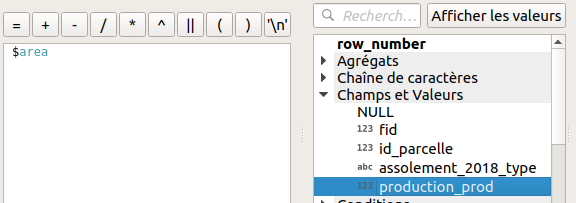
\includegraphics{figures/ajout_champ_production.png}
\caption{Cet outil facilite l'écriture d'expressions}
\end{figure}

Nous connaissons le rendement par type de culture. Nous allons créer un
nouveau champ nommé `production totale',
\texttt{Clic\ droit\ \textgreater{}\ ouvrir\ la\ table\ d\textquotesingle{}attributs}
puis :

\begin{itemize}
\item
  Ouvrir la calculatrice de champ (ctrl+i pour les geeks)
\item
  Cocher \texttt{Créer\ un\ nouveau\ champ}
\item
  Nom : `prod\_totale'
\item
  Type : réel
\item
  La formule à saisir est :

\begin{verbatim}
$area/10000 *  "rendement"
\end{verbatim}
\end{itemize}

Mais attention, dans le cas présenté, la colonne contenant le rendement
(production à l'hectare) par type de culture s'appelle
\emph{``rendement''}. Pensez à bien utiliser l'outil d'aide à la
création d'expression pour retrouver le nom de votre colonne dans la
partie \texttt{Champs\ et\ valeurs} (cf.~image ci-dessus).

\texttt{\$area} représente une fonction qui permet de calculer la
surface du polygone selon l'unité de mesure de la projection utilisée.
Comme nous utilisons du Lambert-93 (EPSG:2154), l'unité est le mètre (ou
mètre carré pour des surfaces). Donc, pour calculer en hectare, nous
divisons la surface en m2 par 10 000 que nous multiplions aussi par le
rendement pour obtenir la production totale.

\subsubsection{Générer le centroïde des
polygones}\label{guxe9nuxe9rer-le-centrouxefde-des-polygones}

Une fois la production totale calculée, nous pouvons générer les
centroïdes des polygones c'est-à-dire, leur centre géographique. Pour
cela, dans la \texttt{boîte\ à\ outils\ de\ traitements}, recherchez le
mot \texttt{centroïdes}, et générez-les (en pensant à bien enregister le
fichier dans un endroit choisi avec un nom compréhensible\ldots{}).

\paragraph{Afficher le type et la production en
étiquette}\label{afficher-le-type-et-la-production-en-uxe9tiquette}

Vous pouvez afficher plusieurs informations dans une étiquette comme le
type d'assolement, sauter une ligne, et la production totale de la
parcelle. Pour cela, on va concatener plusieurs textes (chaînes de
caractères), dont un \texttt{\textbackslash{}n} qui signifie un saut de
ligne.

Dans l'étiquette, saisir l'expression suivante :

\begin{verbatim}
concat("assolement_2018_type",'\n', "prod_totale",'qt')
\end{verbatim}

Pour vous familiariser avec l'outil, vous pouvez remplacer la production
totale par la production à l'ha et afficher une étiquette sous la forme
: \texttt{Maïs\ :\ 89qt/ha}. Rappelez-vous de la différence entre les
simpleset les doubles quotes\ldots{}

\paragraph{Générer les cercles
proportionnels}\label{guxe9nuxe9rer-les-cercles-proportionnels}

Cette étape permet de déterminer la taille d'un symbole en fonction de
la valeur d'un champ. Dans notre cas, nous voulons faire varier la
taille d'un cercle en fonction de la production totale de la parcelle.

\begin{figure}[htbp]
\centering
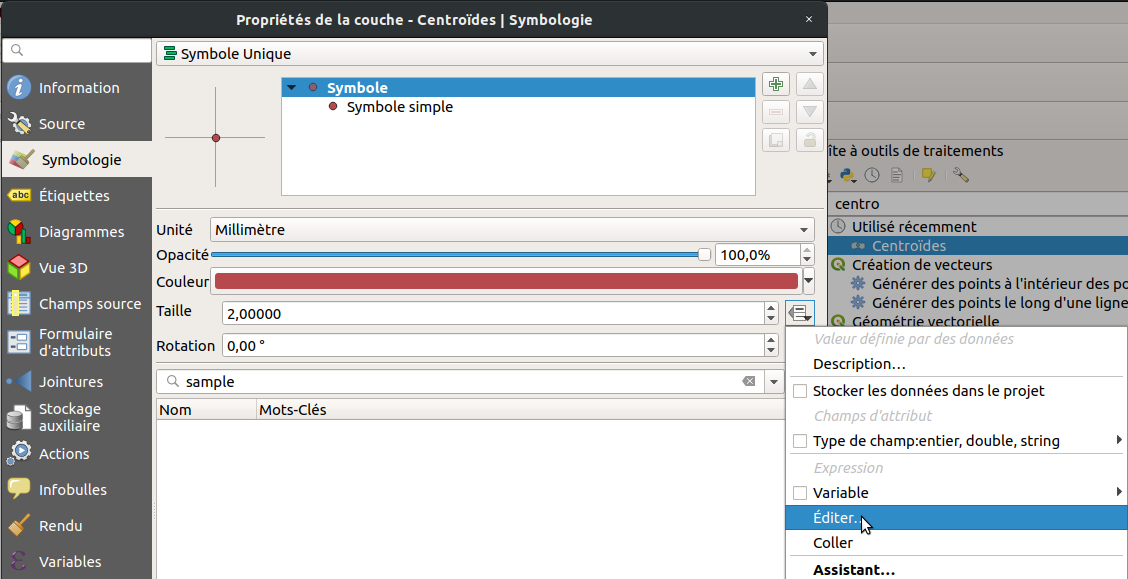
\includegraphics{figures/taille_fonction_champ.png}
\caption{Faire varier en taille en fonction d'une expression}
\end{figure}

Nous devons d'abord choisir une taille minimale et maximale pour
afficher les symboles en faisant en sorte qu'ils ne soient ni trop
petit, ni trop grand pour la carte. Ici, les valeurs de production
totale varient d'environ 200 à plus de 1000 quintaux ce qui est trop
important pour la carte (que ce soit en cm ou en pixels). Nous
choisissons de les diviser par 10 pour pouvoir fixer une taille de
symbole raisonnable. Inutile de créer un nouveau champ : il suffit
simplement, dans le calcul de la taille (clic sur le bouton de droite,
\texttt{Editer}), de le préciser dans une simple expression.

Ainsi, dans la fenêtre de calcul d'expression, quand vous éditez la
taille du cercle (fenêtre symbologie du centroide), vous retrouverez
votre nom de champ dans la partie \texttt{Champs\ et\ valeurs} comme
montré ci-dessous.

\begin{figure}[htbp]
\centering
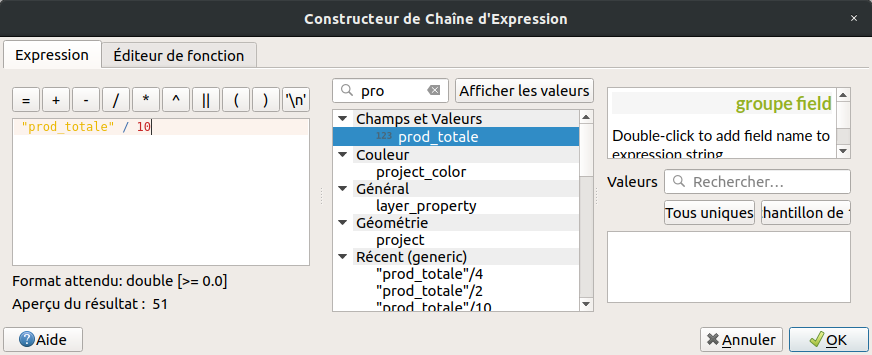
\includegraphics{figures/division_taille_champ.png}
\caption{Utiliser une expression pour calculer la taille du cercle}
\end{figure}

Une fois l'expression calculée, choisissez comme unité de taille le type
\texttt{Point} (fenêtre générale \texttt{Propriétés\ de\ la\ couche}
~\texttt{Symbologie}).

A présent, il faut générer la légende des cercles proportionnels. Pour
cela, toujours dans la partie \texttt{Symbologie}, en bas à gauche,
cliquez sur
\texttt{Avancé\ \textgreater{}\ Légende\ définie\ par\ la\ taille\ des\ symboles}.

\begin{figure}[htbp]
\centering
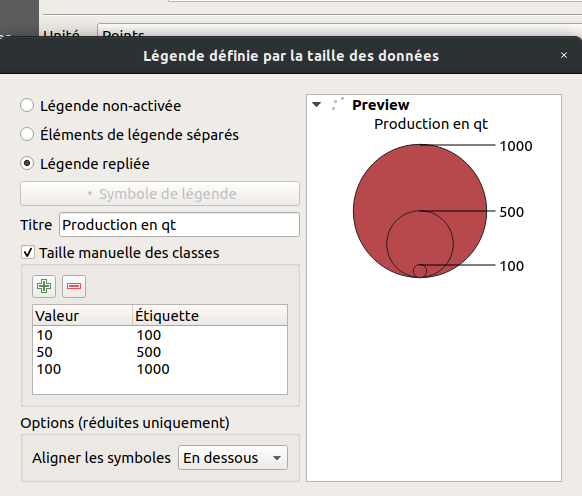
\includegraphics{figures/legend_propor.png}
\caption{Définissez votre légende proportionnelle}
\end{figure}

Pour légender les symboles proportionnels, on utilise ce qu'on appelle
une légende repliée. Il est nécessaire de définir la taille des classes
de manière manuelle car nous avons volontairement divisé par 10 la
taille des cercles. Il y a donc une différence d'un facteur 10 entre la
valeur de taille et la valeur d'étiquette à préciser (relative à la
production totale).

\begin{figure}[htbp]
\centering
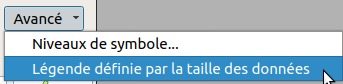
\includegraphics[height=0.52083in]{figures/legend_cercle.png}
\caption{Générer la légende des cercles proportionnels}
\end{figure}

Vous pouvez à nouveau faire une carte en combinant à la fois
l'information ponctuelle (ici la production totale de la parcelle) avec
le rendement selon le type de culture (exemple ci-dessous - erreur à
corriger sur la légende des parcelles).

\begin{figure}[htbp]
\centering
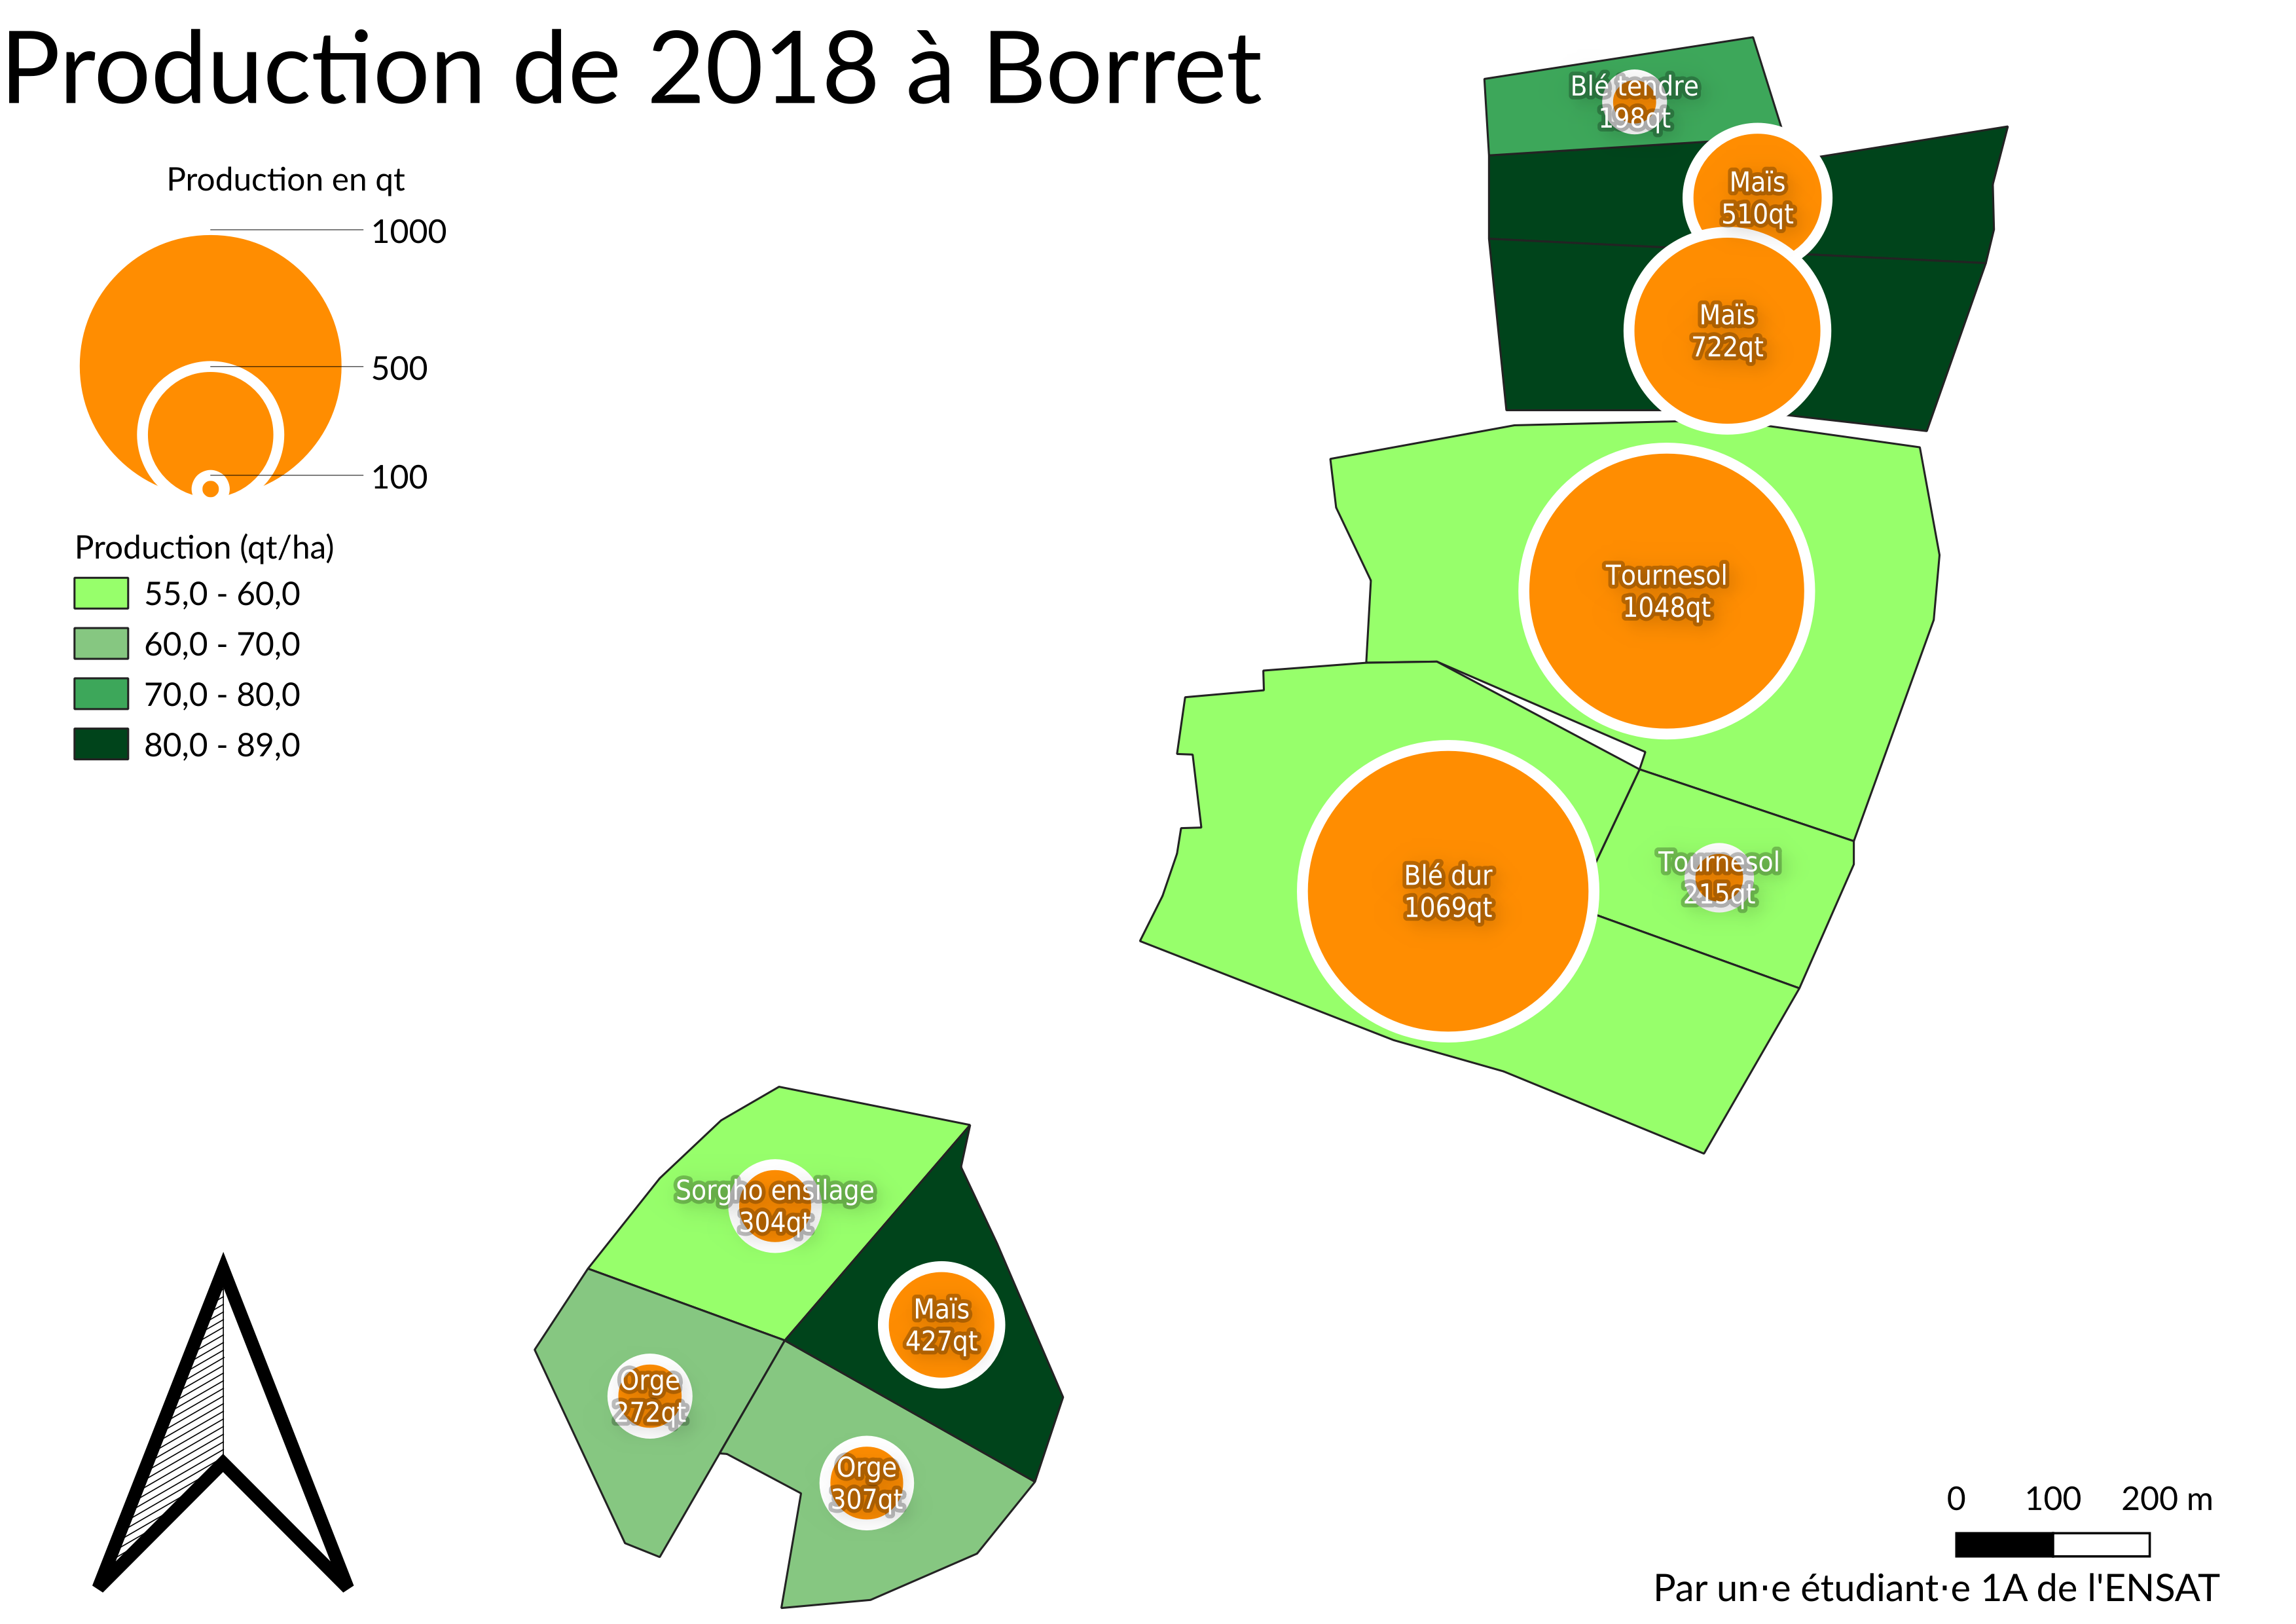
\includegraphics{figures/exemple_proportionnel.png}
\caption{Générer la légende des cercles proportionnels}
\end{figure}

\subsubsection{Ajouter une carte de localisation de la zone
d'étude}\label{ajouter-une-carte-de-localisation-de-la-zone-duxe9tude}

Dans la fenêtre générale de QGIS (hors composeur de mise en page),
ajoutez un fond de carte de type OpenStreetMap (OSM).

Pour ajouter une petite carte (OSM) servant à localiser la zone d'étude
sur votre carte principale, il faut tout d'abord cliquer sur le bouton
\texttt{Ajouter\ une\ nouvelle\ carte\ à\ la\ mise\ en\ page}, comme
pour votre première carte (dans le composeur de mise en page).

Sélectionnez cette nouvelle carte puis, dans
\texttt{Propriétés\ de\ l\textquotesingle{}objet}, allez dans la partie
\texttt{Aperçu} et ajoutez comme cadre votre première carte (celle
contenant vos parcelles).

Pour avoir un style différent de votre carte principale (celle des
parcelles) il faudra faire des allers-retours entre le composeur de mise
en page et QGIS. Par exemple, dans la fenêtre principale de QGIS, mettez
juste le fond OSM et désactivez les couches que vous ne voulez pas voir
(comme vos parcelles) puis, retournez dans le composeur pour
\texttt{Verrouiller\ les\ couches} de votre carte de localisation (dans
l'onglet \texttt{Propriétés\ de\ l\textquotesingle{}objet}). Ainsi,
quand vous remettrez dans le canevas principal de QGIS votre carte des
parcelles, l'aperçu de votre petite carte ne se mettra pas à jour à
gardera uniquement l'ancienne configuration.

\begin{figure}[htbp]
\centering
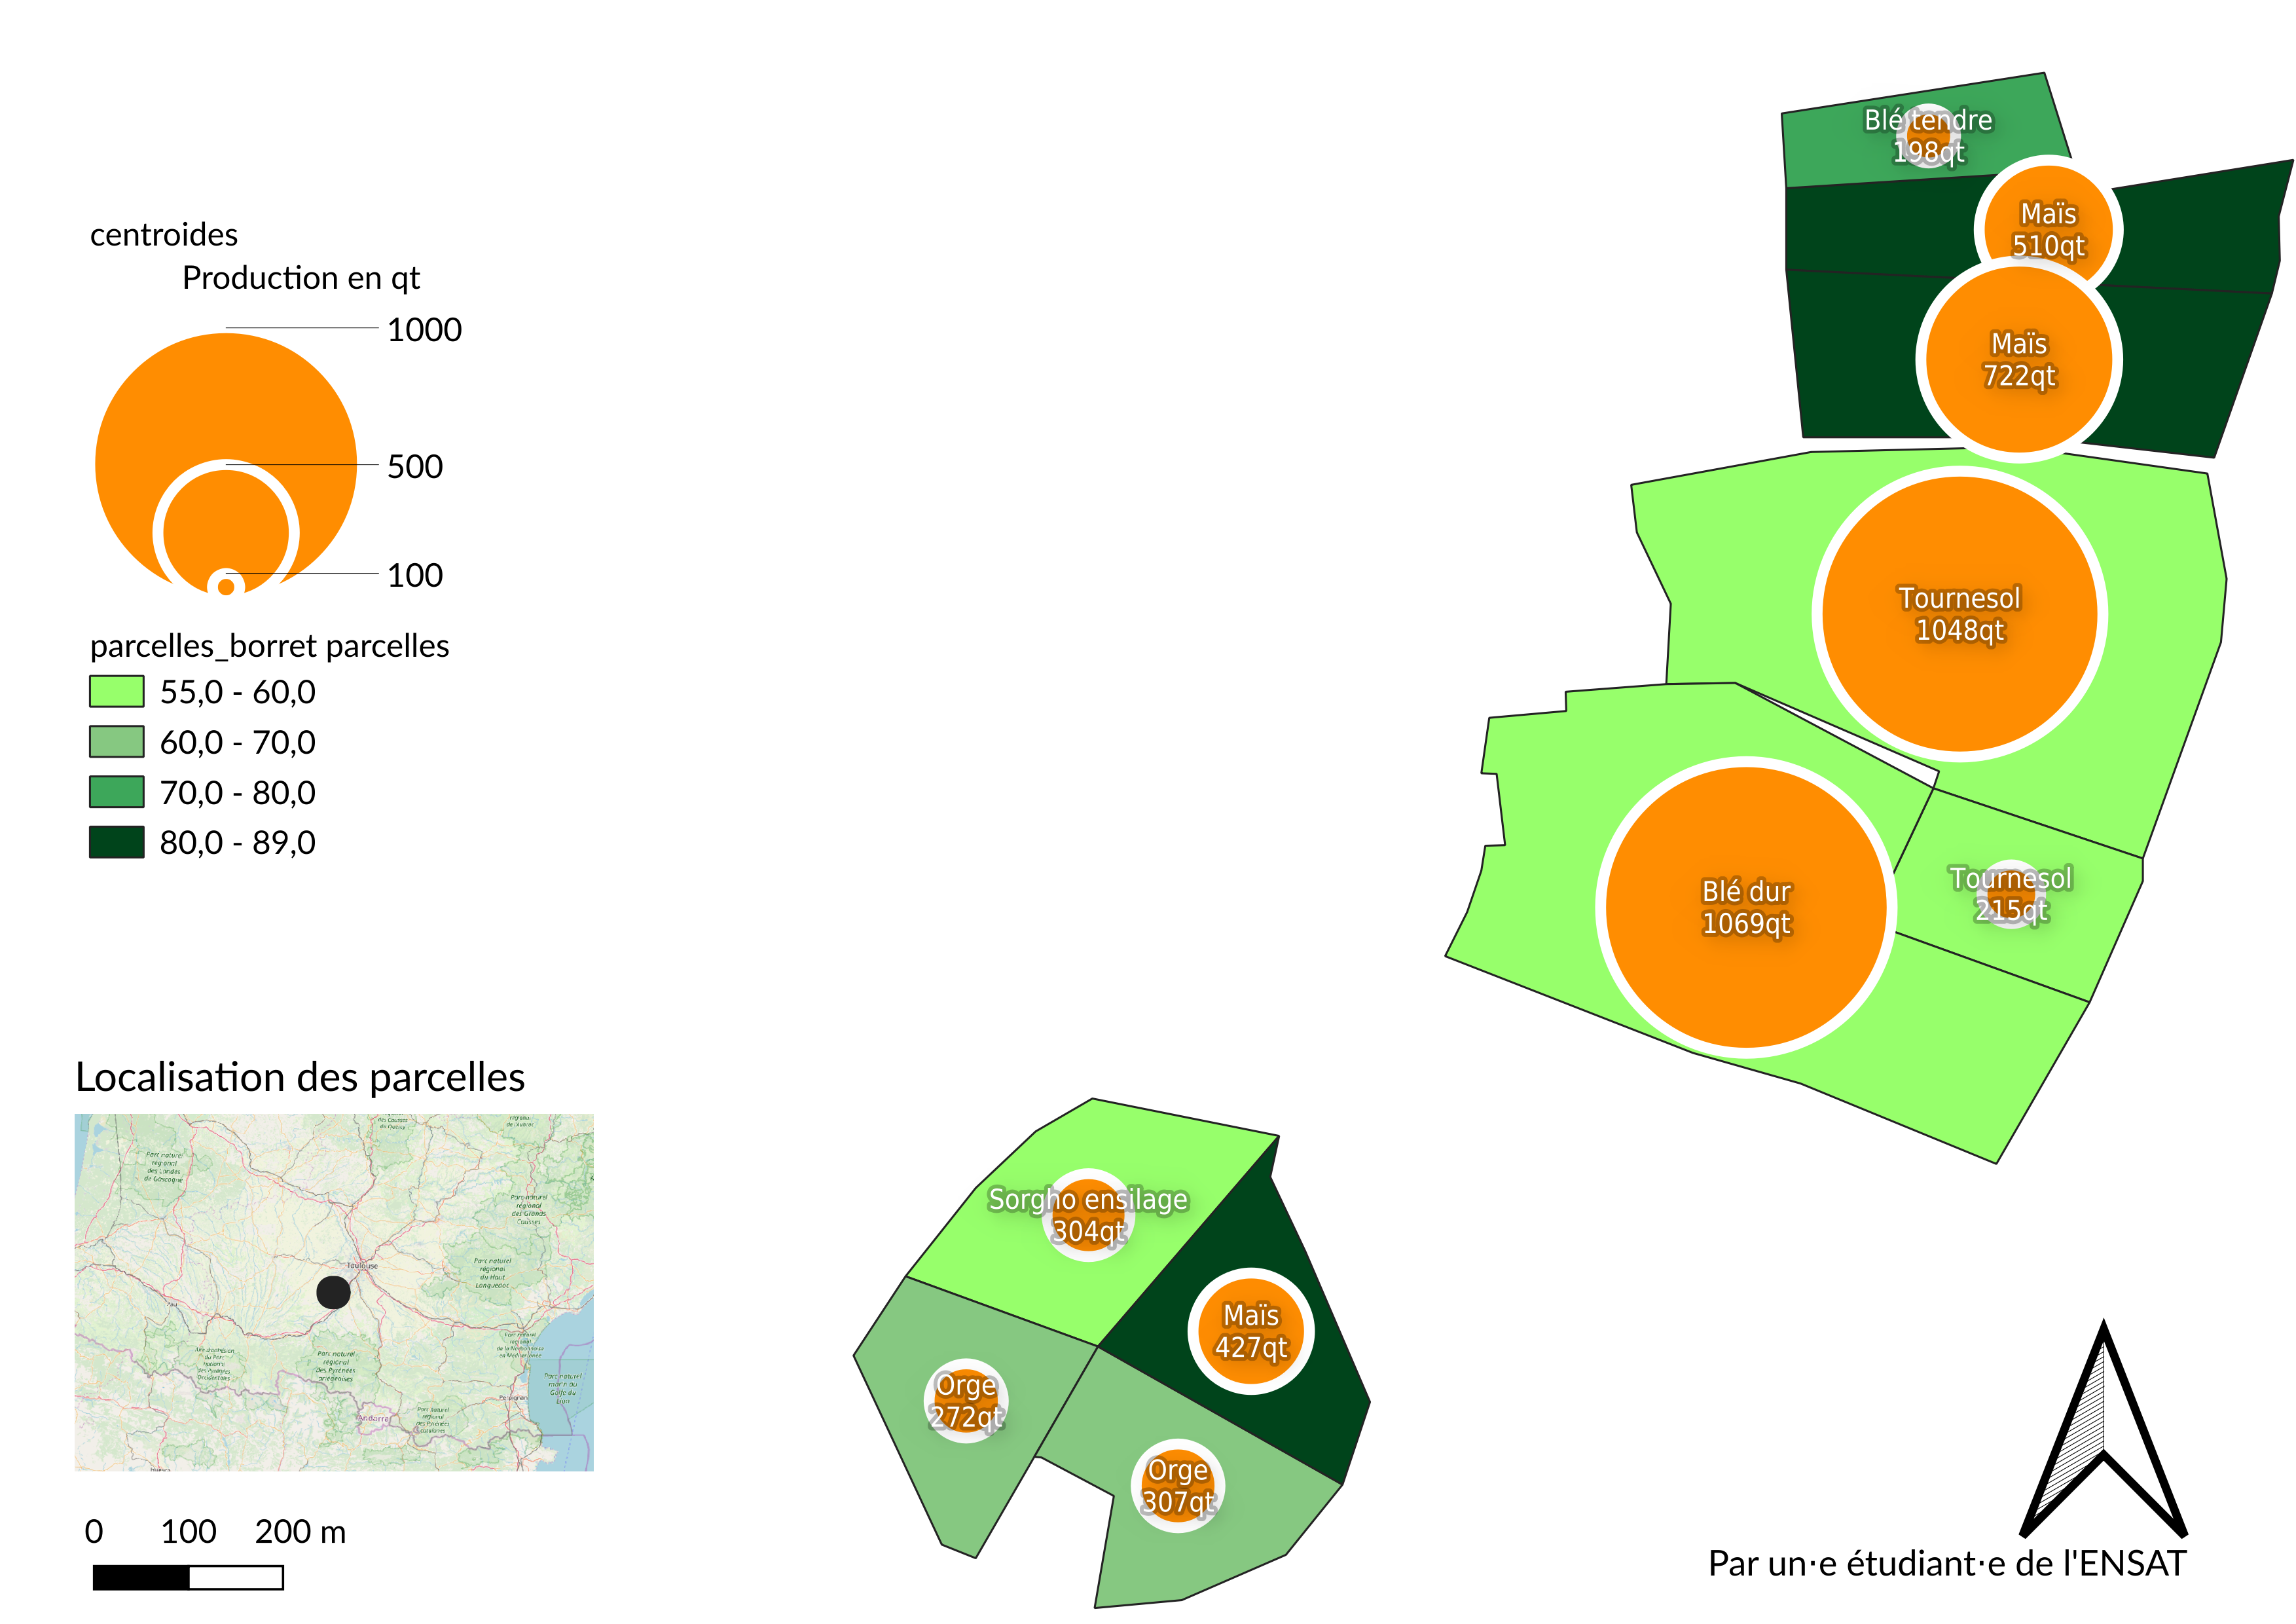
\includegraphics{figures/map_withloc.png}
\caption{Carte avec localisation de la zone d'étude en utilisant des
couches différentes}
\end{figure}

\section{Génération d'un atlas}\label{guxe9nuxe9ration-dun-atlas}

Un atlas permet de générer des cartes détaillées en utilisant un modèle
identique. C'est par exemple utilisé pour préparer un document pour un
relevé sur le terrain en montrant précisément chaque parcelle qui sera
étudiée \emph{in situ}.

L'objectif de l'atlas dans notre cas d'étude est de montrer pour chaque
parcelle sa production totale et d'indiquer le type de culture.

Cliquez sur l'icône \texttt{Paramètres\ de\ l\textquotesingle{}atlas} du
menu du composeur d'impression QGIS puis, cochez dans la fenêtre en bas
à droite \texttt{Générer\ un\ atlas}. La couche de couverture est la
couche pour laquelle chaque entité sera utilisée par QGIS pour générer
chaque page de l'atlas. Nous choisirons ici les polygones des parcelles.

Cliquez ensuite sur votre carte avec l'outil
\texttt{Sélectionner\textbackslash{}Déplacer\ un\ objet} et dans
\texttt{Propriété\ de\ l\textquotesingle{}objet} cochez
\texttt{Controlée\ par\ Atlas}.

Une fois l'atlas créé, sélectionnez votre carte principale (et pas celle
de la localisation), allez dans \texttt{Propriétés\ des\ objets} et
cocher la partie \texttt{Contrôlé\ par\ l\textquotesingle{}atlas}. Vous
pouvez désormais demander à générer votre atlas en cliquant sur le
bouton \texttt{Aperçu\ de\ l\textquotesingle{}atlas}.

\begin{figure}[htbp]
\centering
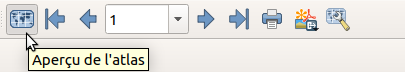
\includegraphics[height=0.62500in]{figures/generate_atlas.png}
\caption{Aperçu de l'atlas}
\end{figure}

Pour ajouter des valeurs (textuelles ou numériques) en fonction de votre
parcelle (comme la production en qt), ajoutez un champ texte (icône
texte sur la gauche), cochez la case \texttt{Rendu\ en\ html} puis
cliquer sur \texttt{Insérer\ une\ expression...}.

Ainsi, il ne sera plus obligatoire d'utiliser la fonction
\texttt{concat} car chaque variable sera mise entre crochets et entre
\%, comme par exemple :

\begin{verbatim}
En 2018, la parcelle n [% "id_parcelle" %] a produit  [% "prod_totale" %] qt de [% "assolement_2018_type" %]
\end{verbatim}

Votre atlas sera donc composé de 10 cartes, dont l'une sera du style :

\begin{figure}[htbp]
\centering
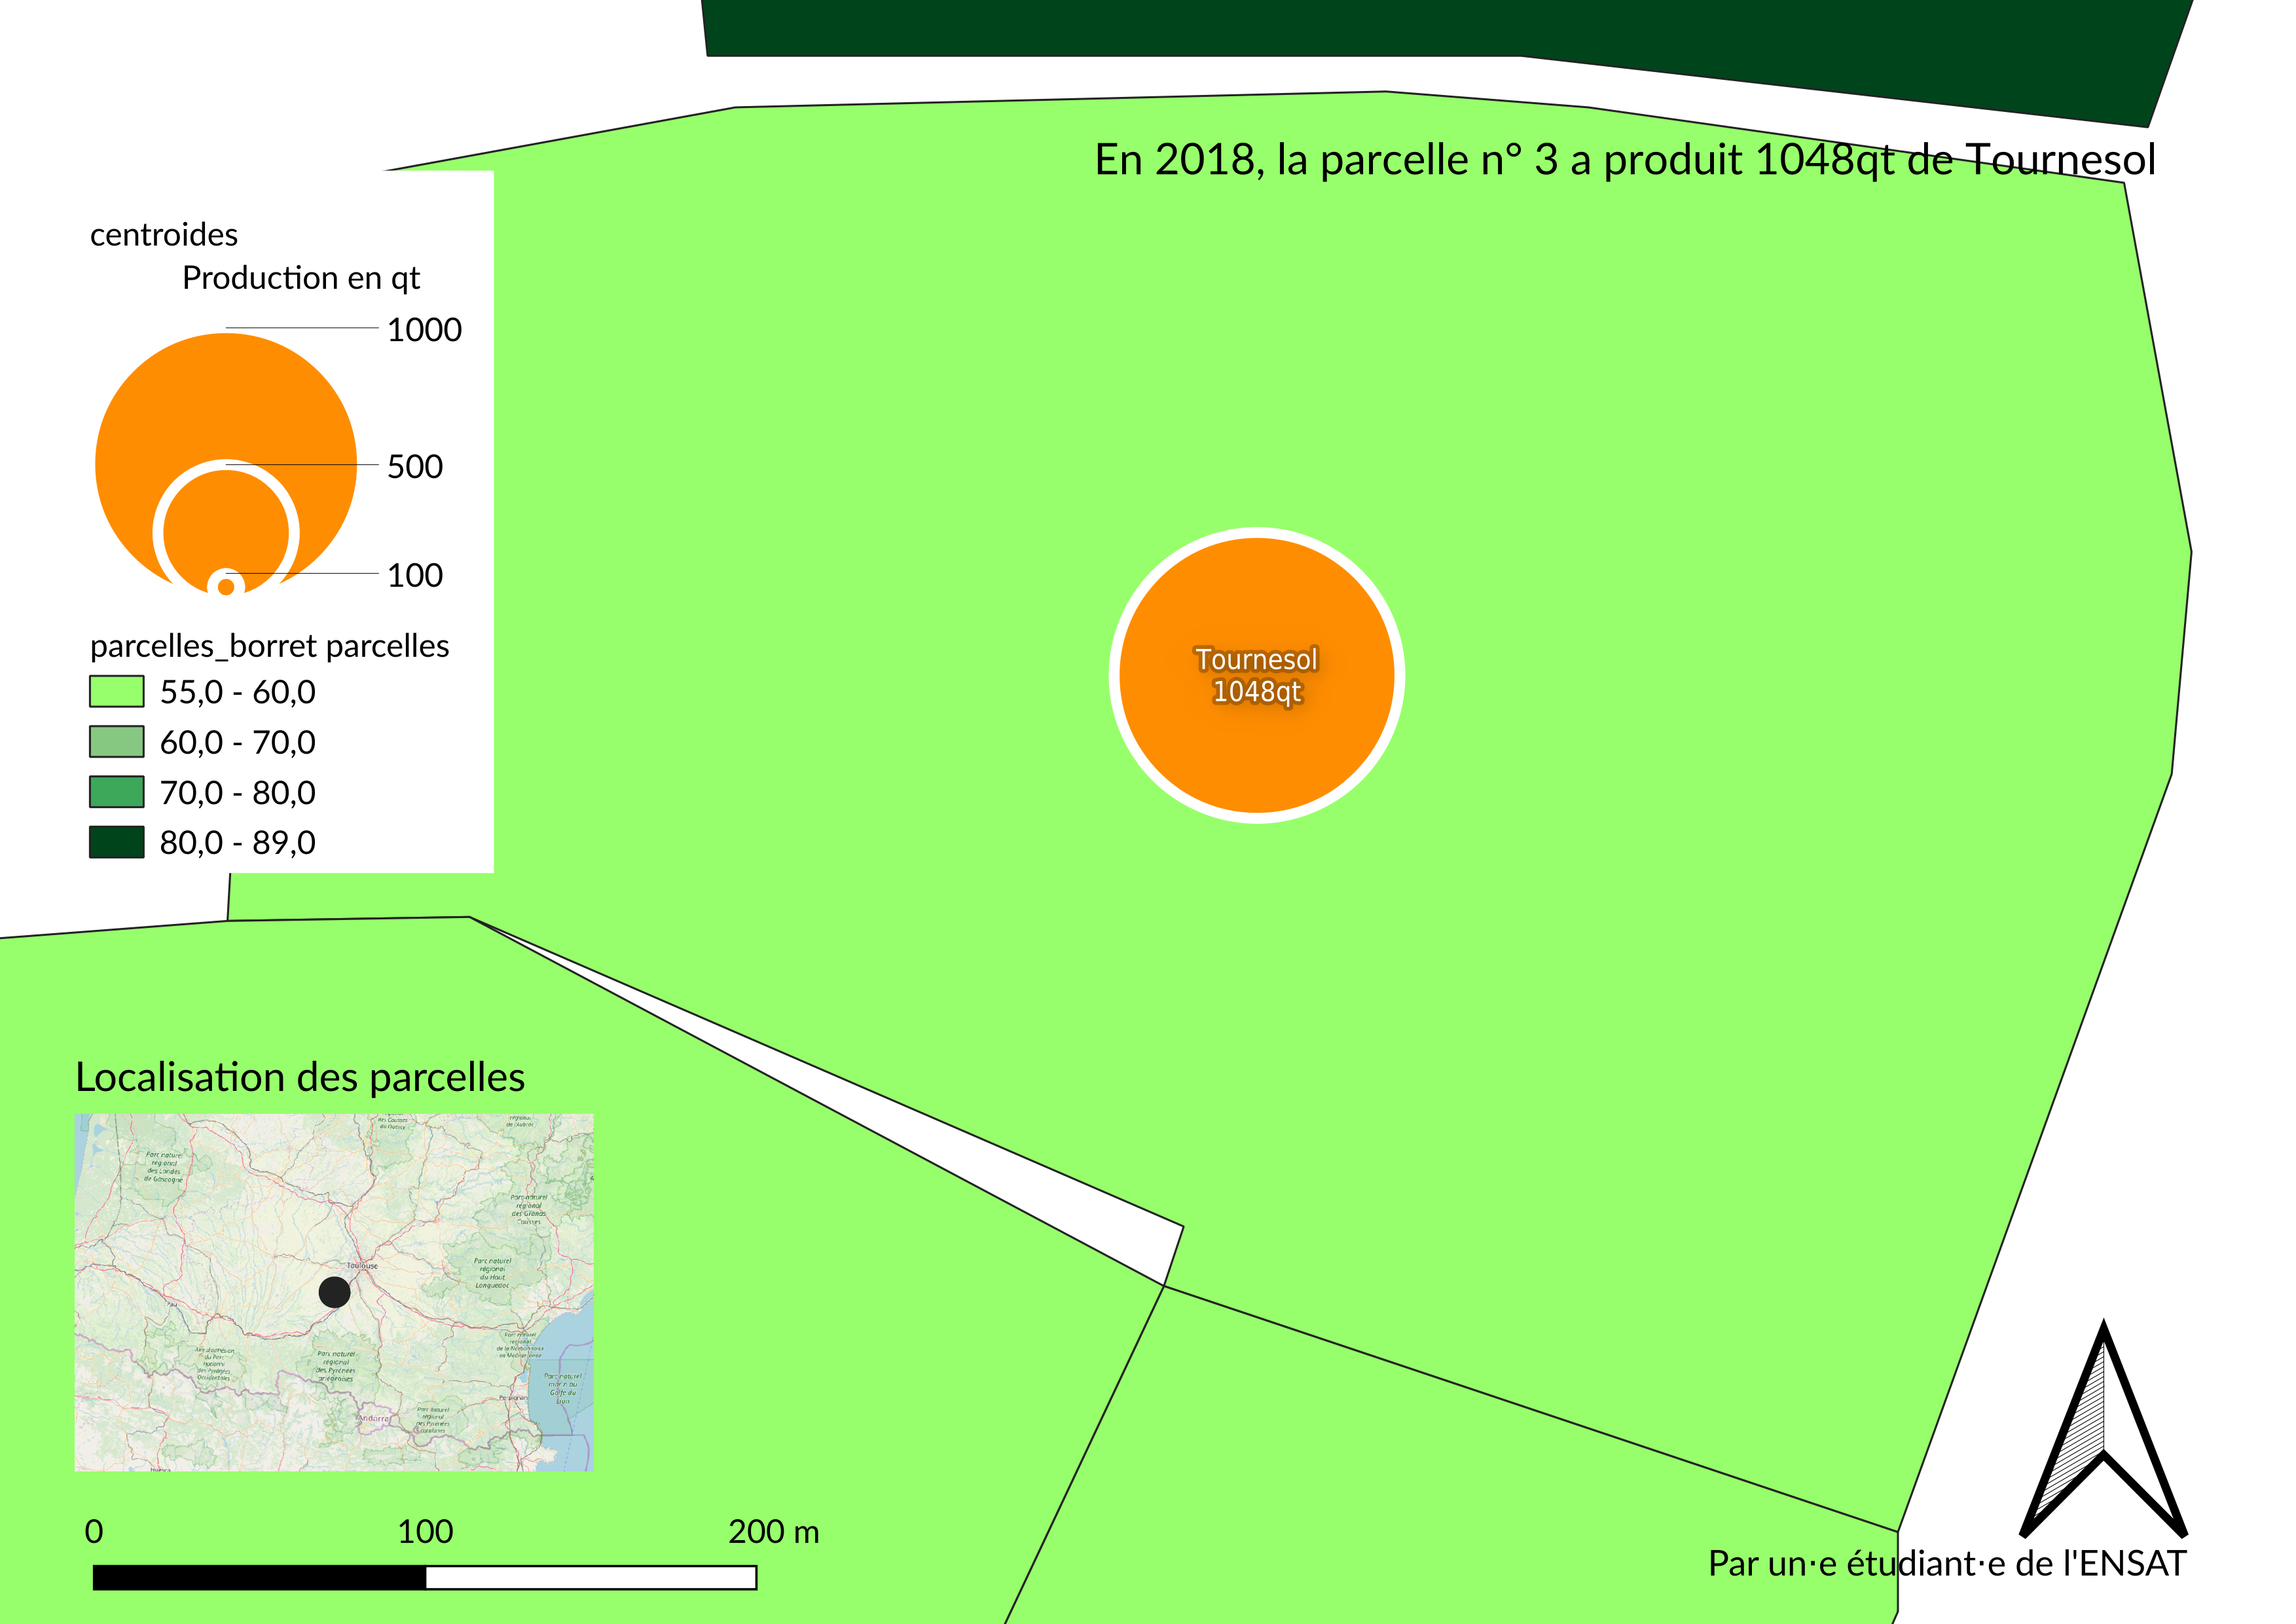
\includegraphics{figures/map_atlas.png}
\caption{Exemple de l'atlas de la parcelle n3}
\end{figure}
